%-------------------------------------------------------------------------------
%                            BAB II
%               TINJAUAN PUSTAKA DAN DASAR TEORI
%-------------------------------------------------------------------------------
\fancyhf{}
\fancyfoot[C]{\thepage}
\chapter{TINJAUAN KEPUSTAKAAN}

\par Untuk mendukung penelitian ini, maka dalam bab ini akan dikemukakan beberapa rumusan teori pendukung yang dikutip dari berbagai referensi baik dalam bentuk buku, jurnal, maupun tulisan karya ilmiah lainnya termasuk hasil penelitian sebelumnya yang ada kaitannya dengan penelitian yang dilakukan.

\section{\textit{MACHINE LEARNING}}
Teknologi \textit{machine learning} (ML) adalah mesin yang belajar atau dilatih dengan menggunakan algoritma dan data tertentu sehingga mesin bisa belajar sendirinya tanpa arahan pengguna. Pembelajaran mesin ini dikembangkan berdasarkan ilmu lainnya seperti statistika, matematika dan \textit{data mining} sehingga mesin dapat belajar dengan analisis data tanpa perlu diperintah oleh pengguna. Dalam hal ini \textit{machine learning} dapat memperoleh data yang ada dengan perintah ia sendiri. \textit{Machine learning} juga dapat mempelajari data yang ada dan data yang ia peroleh sehingga bisa melakukan tugas tertentu. Tugas yang dapat dilakukan oleh ML pun sangat beragam, tergantung dari apa yang ia pelajari \citep{Baker2019}.

\subsection{\textit{Supervised Learning}}
\textit{Supervised Learning} merupakan pendekatan pembelajaran mesin menggunakan set data yang berlabel. Kumpulan data ini dirancang untuk melatih atau "mengawasi" algoritma untuk mengklasifikasikan data atau memprediksi hasil secara akurat. Menggunakan input dan output berlabel, model dapat mengukur akurasinya dan belajar dari waktu ke waktu \citep{Gramejo2020}.

\par \textit{Supervised Learning} dibedakan menjadi dua jenis masalah yaitu klasifikasi dan regresi. Masalah klasifikasi menggunakan algoritma untuk secara akurat menentukan data uji ke dalam kategori tertentu, seperti memisahkan delima dari alpukat. Atau, di dunia nyata, algoritma pembelajaran yang diawasi dapat digunakan untuk mengklasifikasikan spam dalam folder terpisah dari kotak masuk Anda.

\subsection{\textit{Support Vector Machine} (SVM)}
\textit{Support Vector Machine} (SVM) merupakan salah satu metode dalam \textit{supervised learning} yang biasanya digunakan untuk klasifikasi. SVM digunakan untuk mencari \textit{hyperplane} terbaik dengan memaksimalkan jarak antar kelas. \textit{Hyperplane} adalah sebuah fungsi yang dapat digunakan untuk pemisah antar kelas. Pada awalnya SVM dikembangkan untuk persoalan klasifikasi dua kelas, kemudian dikembangkan kembali untuk klasifikasi multi kelas \citep{Braun2011}.

\begin{figure}[H]
	\centering
	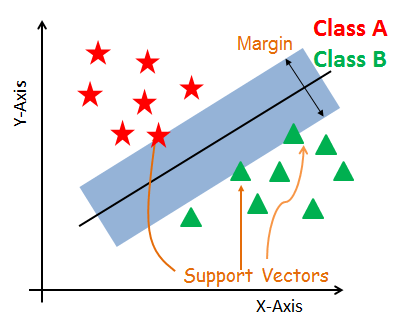
\includegraphics[width=13cm, height=7.3cm]{gambar/index3_souoaz}
	\caption{Support Vectors (Sumber : www.saedsayad.com)}
	\label{index3_souoaz}
\end{figure}


\par Prinsip dasar SVM adalah \textit{linear classifier}. Data pada suatu dataset diberikan variabel xi, sedangkan untuk kelas pada dataset diberikan variabel yi. Metode SVM membagi dataset menjadi 2 kelas. Kelas pertama yang dipisah oleh \textit{hyperplane} bernilai 1, sedangkan kelas lainnya bernilai -1 \citep{Santos2021}. Kedua kelas -1 dan +1 dapat terpisah secara sempurna oleh hyperplane berdimensi d yang didefinisikan:

\begin{equation}
	x_i.w + b = 0
\end{equation}

Data yang termasuk kelas -1 (sampel negatif) dapat dirumuskan sebagai \textit{pattern} yang memenuhi pertidaksamaan:

\begin{equation}
	x_i.w + b = -1
\end{equation}

sedangkan data yang termasuk kelas +1 (sampel positif):

\begin{equation}
	x_i.w + b = 1
\end{equation}

Margin terbesar ditemukan dengan cara memaksimalkan nilai margin antara \textit{hyperplane} dan titik terdekatnya. Hal ini dapat dirumuskan sebagai \textit{Quadratic Programming} (QP) \textit{problem}, yaitu mencari titik minimal persamaan \ref{minimalmargin}, dengan memperhatikan constraint persamaan \ref{constraint}.

\begin{equation}
	min \tau(w) = 1/2||w||^{2}
	\label{minimalmargin}
\end{equation}


\begin{equation}
	y_i(x_i.w + b) - 1 \ge 0
	\label{constraint}
\end{equation}

\par Keterangan:
\par xi = data ke-i
\par w = nilai bobot \textit{support vector} yang tegak lurus dengan \textit{hyperplane}
\par b = nilai bias
\par yi = kelas data ke-i


\par Usaha untuk menentukan \textit{hyperplane} merupakan inti dari proses pembelajaran SVM. \textit{Support vector} adalah titik data yang paling dekat dengan \textit{hyperplane}. Titik-titik ini akan menentukan garis pemisah lebih baik dengan menghitung margin. \textit{Hyperplane} adalah bidang keputusan yang memisahkan antara satu set objek yang memiliki keanggotaan kelas yang berbeda. Margin adalah jarak antara dua garis pada titik kelas terdekat. \citep{Zhibin2008}.


\subsection{\textit{Accuracy, Precision, dan Recall}}
\par Klasifikasi adalah proses pembelajaran secara
terbimbing \textit{(supervised learning)}. Untuk melakukan klasifikasi, dibutuhkan \textit{training set} sebagai data pembelajaran. Setiap sampel dari \textit{training set} memiliki atribut dan kelas label. Namun bagaimana cara mengukur sebuah metode klasifikasi (yang digunakan untuk menentukan kelas label dari sampel baru) memiliki akurasi yang tinggi? \textit{Confusion matrix} merupakan matriks yang menyimpan informasi untuk mengetahui performa dari model yang digunakan dan digunakan sebagai acuan dari performa klasifikasi dari algoritma yang digunakan pada tahap evaluasi \citep{Ariza18}.

% Please add the following required packages to your document preamble:
% \usepackage{multirow}

\begin{table}[H]
	\center
	\fontsize{10}{12}\selectfont
	\caption{\textit{Confusion Matrix}}
	\label{Precision-recall}
	\begin{tabular}{|lc|cc|}
		\hline
		\multicolumn{2}{|l|}{\multirow{2}{*}{}}                 & \multicolumn{2}{c|}{Nilai prediksi}                                \\ \cline{3-4}
		\multicolumn{2}{|l|}{}                                  & \multicolumn{1}{c|}{Positive}       & Negative                     \\ \hline
		\multicolumn{1}{|l|}{\multirow{2}{*}{Nilai sebenarnya}} & Positive                            & \multicolumn{1}{c|}{TP} & FP \\ \cline{2-4}
		\multicolumn{1}{|l|}{}                                  & Negative                            & \multicolumn{1}{c|}{FN} & TN \\ \hline
	\end{tabular}
\end{table}

\par \textit{Confusion Matrix} adalah sumber informasi apakah model yang digunakan berkinerja baik atau tidak. Hal ini bisa dilihat dari nilai yang dari variabel TP \textit{(True Positive)} dan variabel TN \textit{(True Negative)} menunjukkan total prediksi benar yang dibuat oleh model. Sedangkan nilai variabel FP \textit{(False Positive)} dan variabel FN \textit{(False Negative)} menunjukkan total prediksi salah yang dibuat oleh model. Penghitungan kinerja model dapat dilakukan dengan menghitung nilai \textit{accuracy, precision, recall, dan F1-Score} berdasarkan rumus yang terlihat pada persamaan \ref{rumusakurasi}, \ref{rumusprecision}, \ref{rumusrecall}, dan \ref{rumusf1score} \citep{precisionrecall}.

\begin{equation}
	\label{rumusakurasi}
	Akurasi = \frac{TP+TN}{TP+TN+FP+FN}
\end{equation}
\vspace{0.1cm}

\par Secara definisi, \textit{precision} adalah perbandingan antara \textit{True Positive} (TP) dengan banyaknya data yang diprediksi positif. Atau bisa juga dituliskan secara matematis:

\begin{equation}
	\label{rumusprecision}
	Precision = \frac{TP}{TP+FP}
\end{equation}
\vspace{0.1cm}

Sedangkan untuk \textit{Recall}, secara definisi adalah perbandingan antara \textit{True Positive} (TP) dengan banyaknya data yang sebenarnya positif. Dan dapat dituliskan secara matematika seperti ini:

\begin{equation}
	\label{rumusrecall}
	Recall = \frac{TP}{TP+FN}
\end{equation}
\vspace{0.1cm}

Secara definisi, \textit{F1-Score} adalah \textit{harmonic mean} dari \textit{precision} dan \textit{recall}. Yang secara matematik dapat ditulis begini:

\begin{equation}
	\label{rumusf1score}
	F1-Score = \frac{2 \times Precision \times Recall}{Precision+Recall}
\end{equation}
\vspace{0.1cm}

Nilai terbaik \textit{F1-Score} adalah 1.0 dan nilai terburuknya adalah 0. Secara representasi, jika \textit{F1-Score} punya skor yang baik mengindikasikan bahwa model klasifikasi kita punya \textit{precision} dan \textit{recall} yang baik \citep{Ariza18}.


\section{\uppercase{\textit{INDOOR LOCALIZATION SYSTEM} (ILS)}}
\textit{Indoor Localization System} merupakan suatu sistem yang dapat menentukan lokasi \textit{smartphone} yang dimiliki setiap individu di dalam ruangan. Banyak penelitian terkait yang telah dilakukan, diantaranya seperti implementasi \textit{Indoor Localization System} dengan menggunakan pemanfaatan WLAN. Namun, implementasi \textit{Indoor Localization System} dengan menggunakan pemanfaatan WLAN memiliki konsumsi daya baterai yang boros pada \textit{smartphone} \citep{Sun2019}.
\par Solusinya dapat memanfaatkan \textit{Bluetooth Low Energy }(BLE) dalam implementasi \textit{Indoor Localization System}. \textit{Bluetooth Low Energy }(BLE) memiliki konsumsi daya baterai \textit{smartphone} yang lebih sedikit. Terdapat tiga pendekatan dalam \textit{Indoor Localization System}, yakni berdasarkan jarak (trilaterasi), berdasarkan sudut (triangulasi) dan \textit{fingerprinting}. Metode yang digunakan pada penelitian ini adalah metode \textit{fingerprinting}. \textit{Indoor Localization System} sering akurat jika saat mendeteksi sinyal di tempat sunyi, namun akurasi sinyalnya menurun jika terjadi kerumunan\citep{Santos2021}.
%-----------------------------------------------------------------------------%

%\section{\uppercase{CROWDSOURCING INDOOR LOCALIZATION SYSTEM}}

\section{\uppercase{\textit{FINGERPRINTING}}}

\textit{Fingerprinting} adalah teknik untuk menentukan lokasi
yang memanfaatkan \textit{Radio signal strength} (RSS) dari suatu access point. Teknik ini hanya membutuhkan perangkat Wireless LAN dan tidak perlu adanya tambahan perangkat keras lainnya. Fingerprinting melibatkan dua tahapan proses, yaitu tahap training dan tahap positioning. Pada tahapan training dilakukan penyusunan data training yang diambil dari proses survei suatu RSS Access Point
pada suatu lokasi reference point, penentuan reference
point yang saling berdekatan akan mempengaruhi hasil
tahap positioning \citep{Gansemer2010}.

\fancyhf{}
\fancyfoot[R]{\thepage}

\begin{figure}[H]
	\centering
	\shadowbox
	{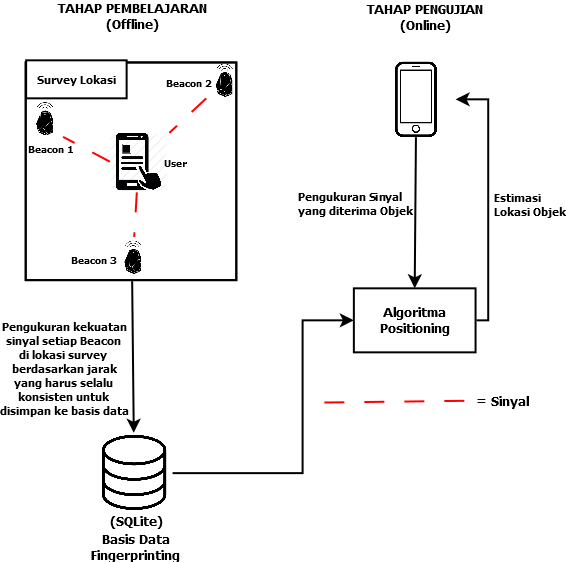
\includegraphics [width = 11cm, height= 9cm]{gambar/fingerprinting}}
	\caption{Ilustrasi Metode \textit{Fingerprinting} }.
	\label{fingerprinting}
\end{figure}

\par Metode \textit{fingerprinting} meliputi dari dua fase, yaitu fase \textit{offline}-dan-fase \textit{online}. Nilai RSS dari beberapa titik referensi yang didapatkan dari \textit{Access Point} dikumpulkan kedalam database dan \textit{radio-map}, fase ini disebut \textit{fase-offline}. Setelah dilakukan \textit{fase offline}, dilakukan penggunaan algoritma sebagai pencocokan data yang telah dikumpulkan menggunakan teknik \textit{fingerprint}, dan fase ini disebut fase \textit{online} \citep{Subhan2011}.

\section{\uppercase{\textit{RECEIVED SIGNAL STRENGTH INDICATOR} (RSSI)}}
\textit{Positioning system} menghasilkan data yang penting untuk menghitung lokasi pengguna. \textit{Time of Arrival} (TOA), \textit{Time Difference of Arrival} (TDOA), \textit{Angle of Arrival} (AOA) dan RSSI adalah metode yang sesuai untuk menghitung data lokasi pengguna untuk kasus \textit{positioning system} \citep{Liu2007}. RSSI menunjukkan kekuatan atau daya yang diterima oleh sinyal \citep{Kajioka2014}. RSSI memperkirakan jarak \textit{node} yang belum diketahui ke referensi node dari beberapa kumpulan unit perhitungan dengan menggunakan atenuasi kekuatan sinyal (\textit{signal strength}) yang dipancarkan dari \textit{transmitter}. Metode ini tepat dilakukan untuk frekuensi sinyal radio \citep{Schneegans2007}.

\par Sebuah nilai RSSI didefinisikan dengan bilangan negatif. Semakin tinggi bilangan negatifnya, maka kekuatan sinyal tersebut tergolong lemah. Namun, jika bilangan nilai RSSI mendekati 0, maka kekuatan sinyal tersebut tergolong kuat. Biasanya, jika suatu objek berada di dekat AP atau \textit{transmitter}, RSSI akan memperoleh nilai yang besar. RSSI dapat digolongkan menjadi 5 kategori kekuatan sinyal seperti terlihat pada Tabel \ref{t_rssi}.

\begin{table}[H]
	\centering
	\caption{Kekuatan Sinyal RSSI \citep{VerisIndustries2013}}
	\label{t_rssi}
	\begin{tabular}{|l|l|l|}
		\hline
		\textbf{No.} & \textbf{Kekuatan Sinyal} & \textbf{Kualitas Sinyal} \\
		\hline
		1.           & Kurang dari -40 dB       & Luar Biasa               \\
		\hline
		2.           & -40 dB hingga -55 dB     & Sangat Baik              \\
		\hline
		3.           & -55 dB hingga -70 dB     & Baik                     \\
		\hline
		4.           & -70 dB hingga -80 dB     & Cukup Baik               \\
		\hline
		5.           & Lebih dari -80 dB        & Buruk                    \\
		\hline
	\end{tabular}
\end{table}

\section{\uppercase{\textit{BLUETOOTH LOW ENERGY} (BLE)}}
\par BLE \textit{Beacon} pada dasarnya adalah sebuah perangkat yang sangat sederhana berupa perangkat \textit{wireless} kecil yang berbasiskan \textit{Bluetooth Low Energy} yang mentransmisikan sinyal radio secara terus menerus yang berkaitan dengan ID dari \textit{beacon} tersebut. Dengan menggunakan \textit{Smartphone} Android terkini, BLE sangat mudah untuk dibaca dan dideteksi. Beberapa informasi yang diperoleh pada pembacaan ini, seperti data sensor dan estimasi jarak antara \textit{beacon} dengan Smartphone. Hanya dengan kedua data tersebut, developer dapat berkreasi untuk mengembangkan banyak aplikasi yang unik, aplikatif, dan dapat bermanfaat untuk optimasi sistem di industri juga manfaat lainnya \citep{Wan2019}.

\par Meskipun BLE \textit{beacon} sangat sederhana, namun, BLE \textit{beacon} dibuat dengan teknologi yang cukup maju. Bluetooth Low Energy, yang merupakan media akses dari \textit{beacon}, memiliki cakupan yang cukup luas (Secara teori 200 m) dari segi jangkauan dibandingkan dengan Wireless Short Range lainnya. Bahkan saat ini dengan berkembangnya \textit{Bluetooth} 5.0, jangkauan \textit{Bluetooth Smart}, menurut Bluetooth SIG, dapat menjangkau 4 kali lipat dibandingkan dengan Bluetooth 4.0. Selain itu, dari sisi \textit{low energy}, teknologi ini menciptakan interaksi seamless yang tidak mengkonsumsi banyak energi baterai (secara teori, dengan baterai 3 volt dapat bertahan selama 2 tahun). Selain itu, oleh karena sistem yang tidak kompleks, teknologi \textit{beacon} tidak perlu bertarung dengan banyak standar aplikasi IoT, sehingga memudahkan developer dalam pengembangannya \citep{Lashkari2018}.

\par Keunggulan BLE dibandingkan \textit{Bluetooth Classic} adalah konsumsi daya baterai dan energi listrik dari BLE untuk \textit{transfer} data jauh lebih kecil dibandingkan dengan \textit{Bluetooth Classic}, tetapi dengan jangkauan konektivitas dan kapasitas pengiriman data yang sama \citep{bluetoothsig2010}. Karakteristik dari BLE adalah ukurannya yang sangat kecil, biaya murah, serta konsumsi daya rendah yang bisa digunakan sampai beberapa tahun ke depan dengan menggunakan jenis baterai AAA \citep{Keluza2017}. Menurut \cite{Paganini2015}, terdapat beberapa platform yang mendukung BLE dan platform tersebut sudah mendukung Bluetooth 4.0. Beberapa platform tersebut adalah sebagai berikut:
\begin {itemize}
\itemsep0em
\item iOS5+ (lebih dianjurkan iOS7+).
\item Android 4.3+ (perbaikan \textit{bug} merous di 4.4+).
\item Apple OS X 10.6+.
\item Windows 8 (XP, Vista dan Windows 7 hanya mendukung Bluetooth 2.1).
\item GNU/Linux Vanilla BlueZ 4.93+.
\end{itemize}

\subsection{\textit{Beacon}}
\par Pada penelitian kali ini, \textit{beacon} yang digunakan adalah merk \textit{KBeacon}. \textit{Beacon} adalah teknologi \textit{Bluetooth Low-Energy} yang dapat digunakan untuk melakukan push notification atau tracking ketika kita sudah berada di jangkauan sinyalnya. Ketika pengguna melewati area di mana sistem penentuan posisi atau jaringan IoT dengan \textit{beacon} diatur, \textit{beacon} terdekat mengirimkan kode dengan pesan ke perangkat seluler mereka. Kemudian, pesan tersebut muncul sebagai pemberitahuan di perangkat seluler pengguna dengan aplikasi seluler pihak ketiga. Ada tiga hal yang harus diperhatikan untuk membuat sistem berbasis \textit{beacon} ini berfungsi, yaitu setidaknya ada satu perangkat \textit{beacon} lagi, aplikasi seluler dan tentunya izin pengguna. Untuk mengaktifkan dukungan \textit{beacon}, ponsel cerdas harus memiliki iOS 7 atau lebih tinggi atau Android 4 atau lebih tinggi. Standar \textit{beacon} Apple disebut \textit{iBeacon}, sedangkan Google bernama Eddystone \citep{Kim2014}.

\par BLE memancarkan sinyal dari alat \textit{transmiter} yang beroperasi menggunakan baterai. Alat \textit{transmiter} tersebut disebut dengan \textit{Beacon}. \textit{Beacon} merupakan alat pendeteksi lokasi dengan harga yang terjangkau, ukurannya yang kecil, memiliki daya tahan baterai yang cukup lama, dan tidak membutuhkan energi listrik tambahan. Setiap perangkat \textit{smartphone} dan \textit{tablets} yang mendeteksi sinyal dari \textit{Beacon}, dapat menghitung jarak dan memperkirakan keberadaan lokasi setiap perangkat sekaligus \citep{Keluza2017}.

\par Kelebihan dari penggunaan \textit{Beacon} diperkirakan bertahan sampai bertahun-tahun hanya dengan energi baterai, serta tahan terhadap debu dan air sesuai dengan standar IP67, dan memiliki ketelitian sejauh 1-3 meter \citep{Insoft2016}. Teknologi BLE merupakan solusi yang tepat yang digunakan pada \textit{Beacon}, karena penggunaan dayanya yang murah, BLE juga termasuk sistem yang ramah lingkungan. Penggunaan daya yang murah pada BLE dicapai dengan menjaga waktu proses transmisi data sesingkat mungkin dan mengizinkan perangkat \textit{smartphone} maupun \textit{tablets} berada pada mode tidur saat proses transmisi data \citep{Feng2011}.



\subsection{\textit{Crowdsourcing}}
\textit{Crowdsourcing} adalah cara memperoleh layanan, ide, dan data berharga dari sekelompok orang, \textit{crowdsensing} adalah definisi yang sama hanya saja data diperoleh oleh perangkat atau sensor dan bukan dari input manusia. Sistem lokalisasi dalam ruangan berbasis Wi-Fi perlu membuat peta radio dengan survei lokasi. Proses survei lokasi memakan waktu dan \textit{crowdsourcing} adalah pilihan yang layak untuk mengatasi masalah ini. Sementara itu, perlindungan privasi telah menarik perhatian dari industri dan akademisi \citep{Li2018}.

\par Crowdsourcing adalah suatu metode untuk  memecahkan masalah yang kompleks dengan bantuan dari sekelompok pengguna, baik secara aktif maupun oportunistik, membantu tugas-tugas yang lebih sederhana. Dengan demikian, crowdsourcing hadir  sebagai solusi untuk mengatasi beban penyiapan awal \textit{Indoor Positioning Systems} (IPS) berbasis \textit{fingerprinting}. Memanfaatkan kemampuan penginderaan smartphone, pengguna anonim dapat mendukung proses konstruksi \textit{fingerprinting} \citep{Santos2021}.

\par \textit{Crowdsourcing} juga mengatasi kelemahan dari \textit{indoor localization system}, dimana jika \textit{indoor localization system} akan mengalami penurunan akurasi jika di keramaian. Oleh karena itu, \textit{crowdsourcing} dalam proses pengumpulan data sinyal dilakukan dengan cara berkelompok atau tidak dengan satu orang, sehingga saat proses \textit{testing} dilakukan dengan \textit{device} apapun, hasil akurasinya akan tetap stabil \citep{Li2018}.

\par Keberhasilan \textit{indoor localization system} berbasis \textit{sistem lokalisasi indoor} sangat bergantung pada data penginderaan \textit{mobile users}, yaitu  tanpa partisipasi \textit{mobile users} yang memadai tidak mungkin diperoleh kinerja yang baik. Tantangan lain yang dihadapi \textit{localization system} berbasis \textit{crowdsourcing} saat ini adalah masalah keandalan dan akurasi lokalisasi. Hal ini terutama karena variasi kekuatan sinyal dalam waktu yang disebabkan oleh pergerakan orang dan furnitur di dalam ruangan \citep{Sun2019}.



\section{\uppercase{ANDROID}}
Android adalah sistem operasi untuk perangkat \textit{smartphone} berbasis Linux \citep{Safaat2011}. Android menyediakan platform \textit{open source} bagi para \textit{developer} untuk menciptakan aplikasi mereka sendiri untuk digunakan oleh bermacam peranti bergerak. Aplikasi Android ditulis dengan bahasa pemrograman Java. Bagaimanapun juga, tanpa menggunakan standar Java Virtual Machine (JVM) sebuah aplikasi Android tidak akan bisa berjalan. Android SDK menyediakan sebuah \textit{tools} dan API untuk mengembangkan sebuah aplikasi pada platform \citep{Sarkar2019}. Menurut \cite{Supardi2011}, ada 4 komponen utama pada aplikasi Android yaitu sebagai berikut:
\begin{enumerate}[1.]
	\itemsep0em
	\item \emph{Activities}, merupakan komponen untuk menyajikan tampilan aplikasi kepada pengguna (\textit{user interface}).
	\item \emph{Service}, merupakan komponen yang tidak memiliki \textit{user interface} atau disebut dengan \textit{layout} pada Android. Namun, \textit{service} ini bekerja dengan cara \textit{background processing}.
	\item \emph{Broadcast Receiver}, merupakan komponen yang berfungsi menerima dan bertugas untuk menyampaikan notifikasi.
	\item \emph{Content Provider}, merupakan komponen yang menangani data secara spesifik sehingga dapat digunakan oleh aplikasi lain.
\end{enumerate}

\section{\uppercase{REACT NATIVE}}
React Native adalah framework JavaScript untuk mengembangkan aplikasi mobile secara multi-platform. Khususnya, pada bagian \textit{front-end} alias interface aplikasi. Sifatnya yang cross-platform memungkinkan satu codebase bisa digunakan di iOS dan Android. Selain itu, React Native juga menghasilkan aplikasi dengan UI/UX mengesankan. Aplikasi bisa berfungsi dengan \textit{smooth} dan komponennya (seperti tombol-tombol) merespon dengan baik layaknya dibuat dengan kode Native \citep{Brito2018}. Cara Kerja React Native cukup simple, yaitu:
\begin{enumerate}[1.]
	\itemsep0em
	\item Developer menggunakan kode React untuk membangun interface aplikasi
	\item Kode React akan diinterpretasikan menjadi JavaScript agar nantinya bisa digunakan untuk aplikasi mobile
	\item React Native akan menggunakan fitur bridge untuk mengolah codebase menjadi Native Module (Android Module, iOS Module)
	\item Native Module siap digunakan di platform yang bersangkutan.
\end{enumerate}z

\section{\uppercase{WEB SERVICES}}
\par \textit{Web service} merupakan aplikasi yang berisi sekumpulan basis data (database) dan perangkat lunak (software) atau bagian dari program perangkat lunak yang diakses secara remote oleh piranti dengan perantara tertentu. Melalui \textit{web service}, memungkinkan pengguna untuk mengatasi permasalahan berupa \textit{interoperability} dan mengintegrasikan sistem berbeda \citep{Chuangwei2011}.

\par Pada umumnya, \textit{web service} memiliki ciri khusus berupa URL layaknya \textit{web}. Yang membuat berbeda adalah interaksi yang diberikan oleh \textit{web service} itu sendiri. URL pada \textit{web service} hanya mengandung sekumpulan informasi, perintah, dan konfigurasi (sintaks yang berguna untuk membangun fungsi tertentu dari aplikasi). \textit{Web service} mampu menukar data tanpa memandang sumber database, bahasa yang digunakan, dan pada platform apa data tersebut dikonsumsi. Kemampuan itulah yang memungkinkan \textit{web service} menjadi jembatan penghubung untuk berbagai sistem \citep{Chuangwei2011}.

\par \textit{Web services} menggambarkan aplikasi yang mengekspos \textit{business logic} sebagai layanan yang menggunakan internet \citep{Mironela2009}. Layanan tersebut dikirim melalui \textit{interface} yang dapat diprogram, sementara fungsionalitasnya dapat dipakai dan dipanggil melalui alamat \textit{Internet Protocol} (IP \textit{address}) \citep{Wagh2012}. \textit{Web services} sering dikategorikan sebagai komponen sistem perangkat lunak yang dirancang untuk mendukung interaksi antar sistem. \textit{Web services} menyediakan informasi atau data pada sistem lain untuk digunakan sebagai fasilitas yang membuat sistem dapat saling berinteraksi. Biasanya, data yang diberikan oleh \textit{web services} berupa data dalam bentuk format JavaScript Object Notation (JSON) atau eXtensible Markup Language (XML) \citep{Rahman2013}. Situs \textit{web} W\textit{orld Wide Web Consortium} (W3C) mendeskripsikan  bahwa \textit{Simple Object Access Protocol} (SOAP), \textit{Representational State Transfer} merupakan protokol yang digunakan \textit{web services} untuk berkomunikasi. Penelitian ini akan menggunakan \textit{web services} dengan layanan protokol REST untuk membantu aplikasi absensi perkuliahan berbasis Android berinteraksi dengan \textit{database} yang terdapat di server.

\subsection{Representational State Transfer (REST)}
REST merupakan hubungan antara klien dan server dan bagaimana sebuah data disimpan. Arsitektur REST didasarkan pada gaya arsitektur klien atau server yang dapat dilihat pada Gambar \ref{restful}. \textit{Request} dan \textit{response} dibangun berdasarkan sumber daya pada saat proses transfer \citep{HaliliRamadani2018}. Konsep dari REST adalah perpindahan antar \textit{state}, dapat dicontohkan seperti sebuah browser yang melakukan permintaan terhadap sebuah halaman situs, maka server akan mengirimkan \textit{state} dari halaman situs tersebut ke browser \citep{Rahman2013}.
\begin{figure}[H]
	\centering
	\shadowbox
	{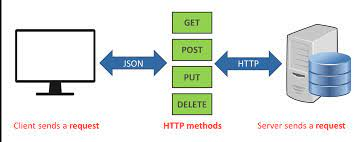
\includegraphics [width = 11cm, height= 4cm]{gambar/restful.jpg}}
	\caption
	{Ilustrasi Arsitektur RESTful dan Komunikasi Antara Klien dan Server \citep{HaliliRamadani2018}}.
	\label{restful}
\end{figure}
\par Navigasi REST dilakukan melalui HTTP untuk melakukan aktivitas tertentu, seolah-olah terjadi perpindahan \textit{state} antara satu halaman dengan halaman lainnya \citep{Rahman2013}. Sebuah aplikasi \textit{web} yang bergantung dengan layanan REST arsitektur disebut dengan RESTful \textit{web services}. RESTful \textit{web services} menggunakan 4 perintah HTTP untuk \textit{create}, \textit{read}, \textit{update} dan \textit{delete} yaitu \textit{GET}, \textit{POST}, \textit{PUT} dan \textit{DELETE} seperti yang terlihat pada Gambar \ref{httprestful} \citep{sinha2014}.
\begin{figure}[H]
	\centering
	\shadowbox
	{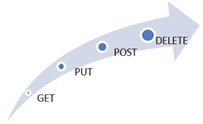
\includegraphics [width = 5cm, height= 3cm]{gambar/httprestful}}
	\caption{Perintah HTTP RESTful \citep{sinha2014}}.
	\label{httprestful}
\end{figure}

\section{\uppercase{SCRUM}}

\par Scrum adalah metode pengembangan perangkat lunak \textit{agile} yang dikembangkan oleh Jeff Sutherland dan tim pengembangannya di awal 1990-an. Prinsip scrum konsisten dengan manifesto agile dan digunakan untuk memandu kegiatan pengembangan dalam suatu proses yang menggabungkan kegiatan kerangka kerja (\textit{framework activity}) berikut: kebutuhan (\textit{requirements}), analisis (\textit{analysis}), desain (\textit{design}), evolusi (\textit{evolution}), dan pengiriman (\textit{delivery}).
\par Dalam setiap kegiatan kerangka kerja, \textit{work task} terjadi dalam pola proses yang disebut \textit{sprint}. Pekerjaan yang dilakukan dalam \textit{sprint} (jumlah \textit{sprint} yang diperlukan untuk setiap kegiatan kerangka kerja akan bervariasi tergantung pada kompleksitas dan ukuran produk) disesuaikan dengan masalah yang dihadapi dan didefinisikan dan sering dimodifikasi secara real time oleh tim Scrum \citep{Ereiz2019}.

% \par \textit{Scrum} pada dasarnya didasari oleh proses model \textit{Incremental} yang merupakan salah satu model pengembangan perangkat lunak. 
\par Dalam metode \textit{Scrum}, seluruh \textit{development cycle} terbagi menjadi sebuah rangkaian iterasi di mana setiap iterasi tersebut merupakan detak jantung dari \textit{Scrum} itu sendiri yang disebut dengan “\textit{Sprint}”.
% Pengerjaan \textit{Sprint} memiliki durasi maksimal selama 30 hari. Karena durasi \textit{Sprint} lebih singkat dibandingkan dengan durasi pengembangan produk, maka dalam produk \textit{development cycle} akan ada beberapa \textit{Sprint}, yang artinya pengembangan produk dengan metode \textit{Scrum} dilakukan secara \textit{Iterative} dan \textit{Incremental} \citep{Mundra2013}. Tahapan-tahapan metode \textit{Scrum} menurut \cite{Schwab2013} adalah sebagai berikut:
\begin {enumerate}[1.]
\item Dimulai dengan mengumpulkan \textit{user requirements}.
% namun tidak harus semua \textit{requirements} diharapkan harus keluar dari pemikiran \textit{user} di tahap awal proses pengembangan. \textit{User} dapat mengubah pikiran mereka di setiap waktu selama proses pengembangan, \textit{user} dapat menambah fitur-fitur baru, menghapus atau memperbarui beberapa fitur yang telah ada sebelumnya.
%%%%%%%%%%%%%%%%%%%%%%%%%%%%%%%%%%%%%%%%%%%%%%%%%%%%%%%%%%%%%%%%%%%%%%%%%%%%%%%%%%%%%%%%%%%%%%%%%%%%%%%%%
\item Tahapan selanjutnya adalah memprioritaskan \textit{requirements} dan \textit{Product Backlog}.
% Sebuah perencanaan yang tepat dalam \textit{Sprint} harus dilakukan sesuai jumlah \textit{Sprint} yang dibutuhkan untuk mengembangkan perangkat lunak, yang terdiri dari durasi \textit{Sprint} tersebut dan \textit{requirements} apa saja yang terdapat di \textit{Product Backlog} yang harus diimplementasikan di setiap \textit{Sprint} (dikenal dengan \textit{Sprint Backlog}).
%%%%%%%%%%%%%%%%%%%%%%%%%%%%%%%%%%%%%%%%%%%%%%%%%%%%%%%%%%%%%%%%%%%%%%%%%%%%%%%%%%%%%%%%%%%%%%%%%%%%%%%%%
\item \textit{Sprint} diawali dengan \textit{Sprint Planning} dimana \textit{Product Owner}, satu orang yang telah diberikan wewenang dan bertanggung jawab untuk memaksimalkan nilai produk di pasar, bertemu dengan tim \textit{Scrum} (tim dengan jumlah 2-9 orang), kemudian bekerja sama untuk memperkirakan \textit{requirements} dari \textit{Product Backlog} apa saja yang dikerjakan selama satu \textit{Sprint}.
%%%%%%%%%%%%%%%%%%%%%%%%%%%%%%%%%%%%%%%%%%%%%%%%%%%%%%%%%%%%%%%%%%%%%%%%%%%%%%%%%%%%%%%%%%%%%%%%%%%%%%%%% 
\item \textit{Sprint Planning} difasilitasi dengan \textit{Scrum Master}. \textit{Scrum Master} adalah seorang pemimpin yang melayani (\textit{Servant Leader}).
% \textit{Sprint Planning} memiliki batasan waktu selama 8 jam di dalam sebuah \textit{Sprint} yang berdurasi selama 30 hari. Keluaran dari \textit{Sprint Planning} adalah daftar pekerjaan dari hasil kesepakatan antara \textit{Product Owner} dan tim \textit{Scrum} dimana pekerjaan itu yang akan dikerjakan oleh tim \textit{Scrum} nantinya selama satu \textit{Sprint} beserta \textit{Sprint Goal} yang dinamakan dengan \textit{Sprint Backlog}.
%%%%%%%%%%%%%%%%%%%%%%%%%%%%%%%%%%%%%%%%%%%%%%%%%%%%%%%%%%%%%%%%%%%%%%%%%%%%%%%%%%%%%%%%%%%%%%%%%%%%%%%%%
\item Setelah \textit{Sprint Planning} berakhir, tim \textit{Scrum} akan mengambil \textit{Sprint Backlog} untuk diri mereka masing-masing dan mengerjakan \textit{Sprint Backlog} setiap hari hingga akhir \textit{Sprint} tanpa campur tangan dari pihak manapun.
% \textit{Daily Scrum} akan dikerjakan oleh tim \textit{Scrum} yang tidak lebih dari 15 menit untuk menentukan apa saja yang akan mereka kerjakan selama 24 jam ke depan berdasarkan perkembangan 24 jam terakhir, serta menyampaikan permasalahan yang menghambat mereka untuk bisa mencapai \textit{Sprint Goal}. Tim \textit{Scrum} akan melakukan perbaikan-perbaikan item dari \textit{Product Backlog} pada \textit{Sprint} yang akan datang selama proses pengembangan berlangsung, dengan tujuan membuat \textit{Sprint Planning} menjadi lebih efektif.
%%%%%%%%%%%%%%%%%%%%%%%%%%%%%%%%%%%%%%%%%%%%%%%%%%%%%%%%%%%%%%%%%%%%%%%%%%%%%%%%%%%%%%%%%%%%%%%%%%%%%%%%%
\item Di akhir \textit{Sprint} saat acara \textit{Sprint Review}, \textit{Product Owner} akan mempresentasikan hasil pekerjaan tim.
% \textit{Scrum} selama satu \textit{Sprint} dan juga menjelaskan apa saja pencapaian tim \textit{Scrum} menuju \textit{Sprint Goal} di dalam \textit{Sprint} tersebut kepada para pemegang kepentingan (\textit{stakeholder}) agar mendapatkan \textit{feedback}. \textit{Feedback} ini akan dimasukkan ke dalam \textit{Product Backlog} agar meningkatkan nilai dari sebuah produk. \textit{Sprint Review} memiliki batasan waktu tidak lebih dari 4 jam untuk \textit{Sprint} yang memiliki durasi selama 30 hari.
%%%%%%%%%%%%%%%%%%%%%%%%%%%%%%%%%%%%%%%%%%%%%%%%%%%%%%%%%%%%%%%%%%%%%%%%%%%%%%%%%%%%%%%%%%%%%%%%%%%%%%%%%
\item Setelah \textit{Sprint Review}, \textit{Scrum Master} memfasilitasi acara yang bernama \textit{Sprint Retrospectives} agar tim \textit{Scrum}, \textit{Product Owner} bekerja sama menentukan apa saja peningkatan yang akan mereka implementasikan di \textit{Sprint} berikutnya.
%  \textit{Scrum Master} yang efektif, akan kreatif dalam memfasilitasi \textit{Sprint Retrospectives}, akan masuk ke dalam \textit{Sprint Backlog} untuk menuju \textit{Sprint} berikutnya. \textit{Definition of Done} adalah salah satu hal yang ditekankan oleh tim \textit{Scrum} pada saat \textit{Sprint Retrospectives}.
%%%%%%%%%%%%%%%%%%%%%%%%%%%%%%%%%%%%%%%%%%%%%%%%%%%%%%%%%%%%%%%%%%%%%%%%%%%%%%%%%%%%%%%%%%%%%%%%%%%%%%%%%
\item \textit{Sprint Retrospectives} merupakan acara yang paling penting dalam \textit{Scrum} dikarenakan sifatnya yang menekankan \textit{continuous learning} yang dapat meningkatkan tingkat \textit{agility} perusahaan. \
% textit{Sprint Review} memiliki batasan waktu tidak lebih dari 3 jam untuk \textit{Sprint} yang memiliki durasi selama 30 hari. Setelah \textit{Sprint Retrospectives} berakhir, maka \textit{Sprint} berikutnya akan langsung dilakukan tanpa ada jeda antar \textit{Sprint}. Pada setiap \textit{Sprint}, \textit{Product Owner} akan memastikan agar produk dapat mencapai nilai setinggi mungkin saat pengembangan produk diakhiri. \textit{Product Owner}, \textit{Scrum Master} dan tim \textit{Scrum} memegang komitmen, keberanian, saling menghargai satu sama lain, keterbukaan dan fokus. Ilustrasi tahapan-tahapan metode Scrum dapat dilihat pada Gambar \ref{scrum} dibawah ini.
\end{enumerate}

\vspace{0,2cm}
\begin{figure}[H]
	\centering
	\shadowbox
	{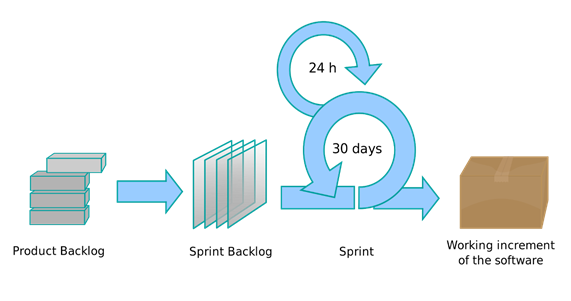
\includegraphics [width = 11cm, height= 5.5cm]{gambar/imagescrum}}
	\caption{Ilustrasi Metode Pengembangan Menggunakan \textit{Scrum} \citep{Schwab2013}}.
	\label{scrum}
\end{figure}


\section{\uppercase{BLACK BOX TESTING}}
Pengujian \textit{black-box} adalah metode pengujian perangkat lunak yang memeriksa fungsionalitas aplikasi tanpa mengintip ke dalam struktur atau cara kerja internalnya. Metode pengujian ini dapat diterapkan secara virtual ke setiap tingkat pengujian perangkat lunak: unit, integrasi, sistem, dan penerimaan. Kadang-kadang disebut sebagai pengujian berbasis spesifikasi. \textit{Black box testing} menurut \citep{Mustaqbal2015} cenderung menemukan hal-hal berikut:
\begin{enumerate}[1.]
	\item Fungsi yang tidak benar atau tidak ada.
	\item Kesalahan \textit{user interface}.
	\item Kesalahan pada struktur data dan akses \textit{database}.
	\item Kesalahan performansi.
	\item Kesalahan inisialisasi dan terminasi.
\end{enumerate}

\section{\uppercase{USABILITY TESTING}}
\par Pengujian kegunaan adalah teknik yang digunakan dalam desain interaksi yang berpusat pada pengguna untuk mengevaluasi suatu produk dengan mengujinya pada pengguna. Ini dapat dilihat sebagai praktik kegunaan yang tak tergantikan, karena memberikan masukan langsung tentang bagaimana pengguna sebenarnya menggunakan sistem. Ini lebih peduli dengan intuitif desain produk dan diuji dengan pengguna yang tidak memiliki paparan sebelumnya. Pengujian tersebut sangat penting untuk keberhasilan produk akhir sebagai aplikasi yang berfungsi penuh yang menciptakan kebingungan di antara penggunanya tidak akan bertahan lama.Ini berbeda dengan metode pemeriksaan kegunaan di mana para ahli menggunakan metode yang berbeda untuk mengevaluasi antarmuka pengguna tanpa melibatkan pengguna.
\citep{Wahl2000}.  \citep{Wesfix2017}.

\par Tujuan lain dilakukannya pengujian ini adalah untuk mengumpulkan data kualitatif yang berhubungan dengan kepuasan pengguna dengan produk yang diuji. Data kualitatif tersebut terdiri dari komentar yang dibuat oleh partisipan, jawaban dari kuesioner pertanyaan dan tanggapan dari partisipan saat proses wawancara. \textit{Usability testing} telah terbukti dapat mengurangi waktu tahap pengembangan, mengurangi jumlah \textit{bugs}, dan menghasilkan produk yang lebih berkualitas untuk meningkatkan nilai jual \citep{Wahl2000}.

\subsection{\textit{Usability Metric for User Experience }(UMUX)} Metode pengujian dengan \textit{usability testing} yang digunakan pada penelitian ini adalah UMUX. \textit{Usability Metric for User Experience} (UMUX) adalah sebuah skala Likert yang mempunyai 4 (empat) item yang digunakan untuk melakukan sebuah penilaian subjektif dari manfaat sebuah aplikasi. UMUX dibuat untuk menghasilkan hasil yang mirip dengan hasil yang diperoleh dengan skala \textit{system usability} yang memiliki 10 item. Selain itu, \textit{Usability Metric for User Experience} (UMUX) cukup ringkas untuk digunakan sebagai modul kegunaan dalam matriks \textit{user experience}. UMUX ditujukan untuk mencocokkan kinerja dari \textit{system usability scale} (SUS) dan penyesuaian dengan langkah-langkah yang lebih penting, UMUX dapat diberikan secara online sebagai survei atau sebagai tindak lanjut dalam pengujian kegunaan, UMUX juga mudah untuk dikelola, karena tidak memerlukan percabangan atau penataan ulang item \citep{Finstad2010}

Adapun daftar pertanyaan-pertanyaan metode UMUX dapat dilihat pada Tabel \ref{tabel-pertanyaan-umux} berikut.
%TABEL PERTANYAAN SUS%
\begin{table}[H]
	\center
	\caption{Daftar Pertanyaan Metode UMUX \citep{Finstad2010}}
	\label{tabel-pertanyaan-umux}
	\begin{tabular}{|l|l|l|}
		\hline
		\rowcolor[HTML]{656565}
		{\color[HTML]{343434} No.} & Pertanyaan                                                                                                                  & Skor \\ \hline
		1                          & Aplikasi ini sesuai dengan kebutuhan saya                                                                                   & 1-7  \\
		\hline
		2                          & Saya memiliki pengalaman buruk dalam menggunakan aplikasi ini                                                               & 1-7  \\
		\hline
		3                          & Aplikasi ini mudah digunakan                                                                                                & 1-7  \\
		\hline
		4                          & \begin{tabular}[c]{@{}l@{}}Saya harus menghabiskan banyak waktu \\ untuk menggunakan aplikasi ini dengan benar\end{tabular} & 1-7  \\ \hline
	\end{tabular}
\end{table}
\begin{comment}
\bibliography{daftar-pustaka}
\end{comment}

\par Adapun hasil dari pengujian UMUX akan dihitung dengan skor pertanyaan ganjil [skor - 1] dan genap [7 - skor]. Total skor kemudian dibagi 24 dan dikali 100 \citep{Finstad2010}. Rumus perhitungan UMUX dapat dilihat pada persamaan \ref{eq:umux}.
\begin{equation}
	\label{eq:umux}
	UMUX = \frac{[P1 - 1] + [7 - P2] + [P3 - 1] + [7 - P4]}{24} x100
\end{equation}
Keterangan:\newline
$P1$ = Pertanyaan satu.\newline
$P2$ = Pertanyaan dua.\newline
$P3$ = Pertanyaan tiga.\newline
$P4$ = Pertanyaan empat.\newline

\par Terkadang hasil dari skor UMUX terlalu positif sehingga perhitungan skor UMUX lebih efektif jika menggunakan UMUX-LITE. UMUX-LITE sendiri memiliki korelasi dalam menghitung skor sehingga untuk menghitung skor UMUX-LITE menjadi SUS dapat menggunakan persamaan \ref{eq:umux-lite} \citep{Borsci2015}.
\begin{equation}
	\label{eq:umux-lite}
	UMUX - LITE = .65(([Item1score] + [Item2score] - 2)100/12) + 22.9
\end{equation}
Keterangan:\newline
$Item1score$ = Pertanyaan satu.\newline
$Item2score$ = Pertanyaan tiga.\newline


\par Hasil skor yang didapat akan dikategorikan menggunakan pedoman SUS. Adapun detail skor skala pada SUS adalah sebagai berikut \citep{Borsci2015} :
\begin{enumerate}[1.]
	\item Grade F (0-51.7)
	\item Grade D (51.8-62.6)
	\item Grade C- (62.7-64.9)
	\item Grade C (65.0-71.0)
	\item Grade C+ (71.1-72.5)
	\item Grade B- (72.6-74.0)
	\item Grade B (74.1-77.1)
	\item Grade B+ (77.2-78.8)
	\item Grade A- (78.9-80.7)
	\item Grade A (80.8-84.0)
	\item Grade A+ (84.1-100)
\end{enumerate}

Hasil pengujian tersebut dapat diukur menggunakan grafik pada gambar \ref{grafikumuxlite}.



\begin{figure}[H]
	\centering
	\shadowbox
	{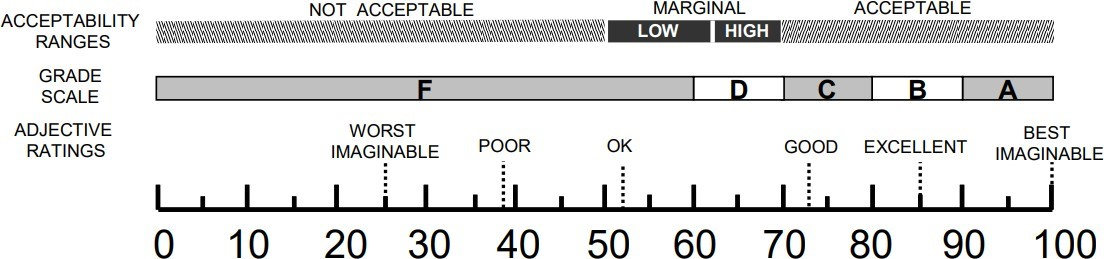
\includegraphics [width = 12cm, height= 4cm]{gambar/umux.jpg}}
	\caption{Perbandingan skala dan skor pada SUS}.
	\label{grafikumuxlite}
\end{figure}